%%%%%%%%%%%%%%%%%%%
% $Id: proj.tex 30 2012-01-06 14:10:38Z aholanda $
%%%%%%%%%%%%%%%%%%
\documentclass[a4paper,12pt,twoside]{article}
\usepackage[]{polyglossia}
\setmainlanguage{brazil}
\setdefaultlanguage{brazil}
\usepackage{graphicx}
\usepackage[top=2.5cm,bottom=2.5cm]{geometry}
\usepackage{hyperref}
\usepackage{setspace}
\usepackage{tikz}
\usetikzlibrary{positioning,shapes}

\def\linux{\href{http://www.kernel.org/}{\sc Linux}}
\def\etal{{et~al.}}
\def\degreelabel{k}
\def\degree#1{\degreelabel(#1)}
\def\degreein#1{\degreelabel^\leftarrow(#1)}
\def\degreeout#1{\degreelabel^\rightarrow(#1)}
\def\vertex{vértice}
\def\hindex{\'indice~$h$}
\def\hdegree#1{h(#1)}
\def\tupla#1{\langle#1\rangle}

\newcommand{\sem}[1]{{\small $#1^o$}}

\newcommand{\keywords}[1]{\noindent{\small {\bf Palavras-chave}: #1.}}

\def\hasmarginpar{0}

\ifnum\hasmarginpar=0
\renewcommand\marginpar[1]{}
\else
\setlength{\marginparwidth}{1.2in}
\let\oldmarginpar\marginpar
\renewcommand\marginpar[1]{\-\oldmarginpar[\raggedleft\footnotesize #1]%
{\raggedright\footnotesize #1}}
\fi

%%%%%%%%%%%%%%%%%%%%%%%%%%%%%%%%%%%%% BEGIN

\pagestyle{myheadings}
\begin{document}

\def\thetitle{Caracteriza\c{c}\~ao das redes complexas formadas pelas
  chamadas de função do sistema operacional \linux}

\title{\thetitle}
\author{Adriano de Jesus Holanda, Zhao Liang} %{$^{*1}$}} \date{\today}
\date{30/8/2017}

\maketitle
\markboth{\scriptsize AJH, ZL}{\scriptsize \thetitle}

\onehalfspacing

\begin{abstract}
  As redes complexas, ou mais genericamente grafos, podem ser
  utilizadas como estrutura para modelar e analisar as
  relações entre elementos de uma variedade de domínios sem uma
  estrutura hierárquica bem definida. Devido ao fato da relação entre
  as funções do código fonte do \linux{} formarem um grafo, torna-se
  adequada para ser modelada como uma rede complexa. Este fato motiva
  este projeto de pesquisa, que tem como objetivo analisar a
  distribuição acumulada dos graus, índice de centralidade e
  coeficiente de agrupamento da redes formadas pelas relações entre as
  chamadas de função de código fonte do sistema operacional (SO) \linux{}. O
  projeto é dividido em 2 (duas) etapas: 1. Análise da variação da
  rede ao longo do tempo de desenvolvimento do sistema; 2. análise do
  comportamento da rede durante a execução do sistema.
\end{abstract}

\keywords{redes complexas, grafos, sistemas operacionais, funções,
  distribuição de graus, centralidade, agrupamento}

% \vfill 
% \begingroup
% \noindent\tt\footnotesize Projeto de Pesquisa na Área de "Engenharia
% de Software e Sistemas de Informação" referente ao concurso público
% para provimento de cargo efetivo de Professor \hbox{Adjunto A} junto à
% UFABC, edital 167/2015.  \endgroup

%% \bigskip
%% \begin{tabular}{l}\hline
%% \noindent {$^*$}Contato: \href{mailto:aholanda@usp.br}{aholanda@usp.br}\\
%% Av. Bandeirantes 3900, CEP: 14040-901, Ribeirão Preto--SP\\
%% $^1$Departamento de Computação e Matemática--DCM\\
%% Faculdade de Filosofia, Ciências e Letras de Ribeirão Preto--FFCLRP\\
%% Universidade de São Paulo--USP\\
%% \end{tabular}

%% \pagebreak
%% \selectlanguage{american}

%% \begin{center}
%% {\Large Characterization of the \linux{} operating system function
%%   invocations as complex network.}\\
%% \bigskip
%% Adriano J. Holanda\\
%% \bigskip
%% \date{\today}
%% \end{center}

%% \bigskip
%% \begin{abstract}
%%   Complex networks, or more generally graphs, can be used to model and
%%   analyze the relations in a wide range of domains without an
%%   hierarchical structure. The relation of function invocation in the
%%   \linux{} source code can be modelled as a complex networks due its
%%   characteristics. Therefore, the aim of the reasearch project is to
%%   analyze the cumulative distribution degree, centrality indices and
%%   clustering coefficient of the network composed by the function
%%   invocations from the source code of \linux{} operating system. Two
%%   subtasks are derived based on the dataset: 1. The analysis of
%%   network changes during the system development; 2. the network
%%   differences between static (source code) and dynamic (runtime) when
%%   the operating system is executing.
%% \end{abstract}

%% \bigskip
%% \noindent\textbf{Keywords:} complex networks, graphs, operating system, function,
%% cumulative degree distribution, centrality, clustering.

%% \vfill

\selectlanguage{brazil}
%2) Enunciado do problema: Qual será o problema tratado pelo projeto e
%qual sua importância? Qual será a contribuição para a área se bem
%sucedido? Cite trabalhos relevantes na área, conforme necessário.
\section{Enunciado do problema}


%% MELHORAR MUITO VAGO
A análise de um sistema computacional de grande porte como o \linux{}
é uma tarefa de difícil execução devido à complexidade do código
fonte, e por consequência, da relação entre as interações do sistema
em tempo de execução. Apesar de conjuntos de testes como o
\textit{Linux Test
  Project}\footnote{\url{http://ltp.sourceforge.net/}} serem
importantes para a identificação de erros, eles não fornecem dados
sobre a influência da alteração do código fonte nas relações entre
seus componentes, que poderiam auxiliar no entendimento da estrutura
do sistema. O problema passa a ser então definir um conjunto de
medidas, aplicá-las e analisar os resultados para identificar o efeito
que alterações no código podem produzir em sua estrutura e nas
interações dos seus componentes com o sistema em execução.

As redes complexas têm sido aplicadas a conjunto de dados de diversos
contextos ou domínios tais como linguística~\cite{cnet:thesaurus},
culinária~\cite{cnet:culinary}, biologia molecular~\cite{huber-2007},
estrutura global de transporte aéreo~\cite{guimera-2005}, dentre
outros. São consideradas redes complexas os grafos que possuem as
seguintes características: grande quantidade de vértices, esparso,
propriedades de mundo pequeno (\textit{small word}) e distribuição de
graus baseada em uma lei de potência~\cite{chung2006}.

Devido ao fato das redes complexas possuírem as características
citadas anteriormente, elas podem ser aplicadas no código fonte e no
sistema em execução do \linux{} para extrair propriedades que auxiliem
sua caracterização. Por este motivo, este projeto de pesquisa tem como
objetivo estudar as relações nas redes formadas pelo conjunto das
invocações de funções do sistema operacional \linux{} utilizando a
distribuição acumulada dos graus, índice de centralidade dos vértices
e coeficiente de agrupamento como parâmetros.

O estudo mais similar encontrado na
literatura\footnote{\label{search}De acordo com pesquisa realizada
pelo autor no Google Scholar (\url{http://scholar.google.com}) em
novembro de 2015.} foi realizado por Wang~\etal~\cite{wang2009}, que
analisaram os módulos de sistemas de arquivos e \textit{drivers} de
223 versões do \linux{} como um rede complexa. Porém, outros módulos
importantes, tais como escalonamento, não foram analisados e não houve
análise com o kernel em execução. Este projeto de pesquisa pretende
estender a análise para outros módulos, calculando alguns
índices de centralidade e adicionando a dinâmica de execução no estudo.

\subsection{Trabalhos relevantes na área}

O primeiro$^{\ref{search}}$ trabalho de aplicação de redes complexas em sistemas
computacionais foi realizado por Clark e Green~\cite{zipf:lisp}, que
analisaram 5 programas feitos em LISP e verificaram que a distribuição
da frequência dos átomos seguem a lei de Zipf, ou seja, o enésimo
termo é $n^{-1}$ tão frequente quanto o termo mais comum. Os autores
sugeriram que o conhecimento desta distribuição poderia guiar o design
do esquema de distribuição da distância entre os ponteiros para
átomos.

Potanin \etal~\cite{potanin:oop_scale_free} analisaram 60 redes
formadas pelo relacionamento entre as classes da linguagem de
programação Java de 35 programas diferentes, mostrando que a
distribuição de frequência dos graus de entrada e saída dos vértices
não possui escala ({\em scale free})~\cite{barabasi-science-2009},
seguindo uma lei de potência com um expoente aproximado de $-2$.

% ?? explicar o q é small word ??
Valverde \etal~\cite{valverde-2002} obtiveram resultados semelhantes a
Potanin analisando o Kit de Desenvolvimento Java 1.2 (JDK 1.2) com a
frequência acumulada dos graus seguindo um lei de potência com
expoente $-2.85\pm 0.11$, sugerindo que o comportamento sem escala
da distribuição ocorreu devido ao processo de otimização local dos
componentes do Kit ao longo do tempo.

Zheng~\etal~\cite{zheng2008} analisaram as dependências entre os
pacotes de programas da distribuição \linux{} \textit{Gentoo} e
econtraram um ajuste através da exponencial estendida para a
distribuição dos graus dos nós. Também propuseram dois novos modelos
para a formação da rede que se ajustasse mais adequadamente a
probabilidade de anexação preferencial e envelhecimento dos nós.

Wang \etal~\cite{wang2009} analisaram os módulos de sitemas de
arquivos e \textit{drivers} de 223 versões do kernel do Linux como uma
rede complexa. A distribuição de graus dos grafos formados pelas
invocações das funções apresentaram propriedades de mundo pequeno,
sem escala e forte anexação preferencial. 

%% 3) Resultados esperados: O que será criado ou produzido como resultado
%% do projeto proposto?

%% 4) Desafios científicos e tecnológicos e os meios e métodos para
%% superá-los: explicite os desafios científicos e tecnológicos que o
%% projeto se propõe a superar para atingir os objetivos. Descreva com
%% que meios e métodos estes desafios poderão ser vencidos. Cite
%% referências que ajudem os assessores que analisarão a proposta a
%% entenderem que os desafios mencionados não foram ainda vencidos (ou
%% ainda não foram vencidos de forma adequada) e que poderão ser vencidos
%% com os métodos e meios da proposta em análise.

\section{Metodologia}
\label{s:metodologia}

\subsection{Preparação dos dados}
\label{s:preparacao}

O conjunto de dados do estudo será composto pelo código fonte do
sistema operacional \linux. Os critérios de escolha para o sistema
operacional foram:

\begin{enumerate}
  \item Código fonte aberto;
  \item Ser utilizado em produção;
  \item Código fonte disponível desde as versões iniciais do sistema.
\end{enumerate}

O código fonte do sistema será baixado a partir da versão {\tt 1.0}
até a versão mais recente ({\tt 4.x} no período da escrita deste
projeto). As versões a serem estudadas, {\tt 1.0, 1.1, 1.2, 1.3, 2.0,
  2.1, 2.2, 2.3, 2.4, 2.5, 2.6, 3.x, 4.x},\ são as versões tradicionais
do sistema.

Alguns ajustes terão que ser feitos para a possibilidade de análise
comparativa, sendo o primeiro a normalização e outro provável é a
construção de um dicionário de sinônimos para as funções, pois muitas
delas sofrem alteração de seu nome ao longo do desenvolvimento.

Os arquivos de cabeçalho que compõem o núcleo do sistema serão
utilizados para seleção das funções a partir de seus protótipos.
Será feita uma filtragem das funções que não realizarem tarefa
relacionada ao subsistema em que forem invocadas. Por exemplo, os
arquivos dos programas que compõem o subsistema escalonador do
\linux{} começam com {\tt sched*}; as funções que não estiverem
relacionadas ao escalonamento ou auxílio a este serão excluídas do
conjunto de dados. Funções auxiliares, como as que geram um diário
({\em log}) da sequência de tarefas realizadas não serão incluídas no
conjunto de dados.

As funções serão classificadas de acordo com a divisão de tarefas
tradicionais para os sistemas operacionais, ou seja, os
subsistemas. Por exemplo, a seguinte classificação poderá ser
realizada:

\begin{enumerate}
\item Gerenciamento de processos: serão agrupadas as funções que lidam
  com a execução dos programas e gerenciamento dos recursos de
  hardware de forma que o processador fique o menos ocioso possível e
  que o tempo de espera do usuário seja pequeno.

\item Gerenciamento de memória: serão agrupadas as funções que
  controlam as tarefas de alocação e troca ({\em swapping}) com o
  disco.
  
\item Controle de entrada e saída: agrupará as funções que gerenciam
  dispositivos periféricos. No caso dos sistemas baseados na
  arquitetura Unix, estas funções lidam com manipuladores de arquivos
  e {\em drivers} de dispositivos.
  
\item Sistema de arquivos: funções específicas de gerenciamento físico
  dos arquivos e suas propriedades serão agrupadas nesta categoria.

\item Outras: funções essenciais não classificadas nas categorias
  anteriores e outras que não possuírem funções correlatas que
  permitam formar um agrupamento separado.
\end{enumerate}

Esta classificação poderá ser alterada ao longo do estudo conforme a
análise dos códigos dos sistema operacionalfor se
aperfeiçoando. Portanto, ela serve apenas como um guia inicial sem a
pretensão de ser definitiva ou exaustiva.

O estudo do código fonte fornece-nos uma caracterização estática da
rede. Para verificarmos a dinâmica da rede em função do tempo de
execução do sistema, as mensagens do núcleo serão armazenadas para
obtenção das medidas e verificação das diferenças quando comparadas
com as medidas das redes estáticas. As redes serão formadas a partir
dos dados obtidos da versão mais recente, no momento de execução do
projeto, do \linux{}, devido à dificuldade de executar versões mais
antigas.

Em resumo, haverá comparação entre as distribuições de graus,
centralidade e agrupamento classificando as redes de acordo com:

\begin{enumerate}
\item A versão do código fonte a ser analisado;
\item Com o estado dos elementos, podendo ser este estático (código
  fonte) e dinâmicos (em execução) e somente da versão mais recente do
  núcleo do \linux.

\end{enumerate}


\noindent{{\bf Representação e construção do dígrafo (grafo
  direcionado)}}\smallskip

  Para a construção do dígrafo $G^\rightarrow(V,E)$ será adotada a
  seguinte convenção: as funções serão os vértices $V$ e os arcos $E$
  irão da função que invoca em direção à função que é invocada.  Como
  exemplo, a Figura~\ref{fig:function} mostra o subdígrafo construído
  extraindo as funções {\tt resched\_task} e {\tt resched\_cpu} do
  escalonador (arquivo {\tt kernel/cpu/sched.c}) do kernel do Linux
  (versão 2.6.29).

 \begin{figure}[ht]
   \centering
   \usetikzlibrary{shapes,positioning}
\begin{tikzpicture}[mynode/.style={ellipse,draw},myedge/.style={->,>=latex}]
  \node[mynode] (resched) {\scriptsize\tt resched\_cpu};
  \node[mynode] (rq) [below=of resched] {\scriptsize\tt cpu\_rq};
  \node[mynode] (task) [below left=of resched] {\scriptsize\tt resched\_task};
  \node[mynode] (spin) [below left=of task] {\scriptsize\tt assert\_spin\_locked};
  \node[mynode] (smpmb) [below=of task] {\scriptsize\tt smp\_mb};
  \node[mynode] (irq) [below right=of task] {\scriptsize\tt spin\_locked\_irqsave};
  \draw[myedge] (resched) -- (rq);
  \draw[myedge] (resched) -- (task);
  \draw[myedge] (task) -- (smpmb);
  \draw[myedge] (task) -- (spin);
  \draw[myedge] (task) -- (irq);
\end{tikzpicture}

   \caption{Subdígrafo direcionado das funções {\tt resched\_task} e
     {\tt resched\_cpu} do escalonador do kernel do Linux versão
      $2.6.29$.}
   \label{fig:function}
 \end{figure}

 O subgrafo conteria o conjunto de vértices $$\{resched\_cpu,
 resched\_task, cpu\_rq, spin\_trylock\_irqsave\}$$ e o conjunto de
 arcos $$\{\tupla{resched\_cpu,resched\_task}, \tupla{resched\_cpu,cpu\_rq},$$
 $$\tupla{resched\_cpu,spin\_trylock\_irqsave}\}$$.
 
\subsection{Caracterização da rede}
\label{s:medidas}

A partir dos gráficos construídos conforme descrito na Seção
\ref{s:preparacao} serão efetuados 3 tipos de medidas:

\def\dist{Distribui\c{c}\~ao acumulada dos graus dos v\'ertices}
\def\centr{Índice de centralidade dos v\'ertices}
\def\group{Coeficiente de agrupamento}

\begin{enumerate}
\item \dist;
\item \centr;
\item \group.
\end{enumerate}

\subsubsection{\dist}
\label{s:distribuicao}

Para o dígrafo $G^{\rightarrow}(E,V)$, o grau de cada vértice pode ser
obtido a partir da matriz de adjacência. Para o grau de saída

\begin{displaymath}
  \label{eq:k}
  \degreeout{v} = \sum_{w \in V} {a^\rightarrow(v,w)},
\end{displaymath}


\noindent onde ${a^\rightarrow(v,w)} = 1$ se $(v,w) \in E$ e $0$ caso contrário, 
 e para o grau de entrada

\begin{displaymath}
  \label{eq:kin}
    \degreein{v} = \sum_{w\in V} a^\leftarrow(v,w).
\end{displaymath}

O grau médio dos vértices é uma medida de conectividade global da
rede, onde

\begin{displaymath}
  \label{eq:avgin}
    \degreein{G} =  {1 \over |V|} \sum_{v\in V}\degree{v},
\end{displaymath}

\noindent é a média para os graus de entrada,

\begin{displaymath}
  \label{eq:avgout}
   \degreeout{G} =  {1 \over |V|} \sum_{v\in V}\degreeout{v},
\end{displaymath}

\noindent é a média para os graus de saída,

\begin{equation}
  \label{eq:avg}
   \degree{v} =  \degreeout{v}  + \degreein{v} 
\end{equation}

\noindent é a média total dos graus dos vértices da rede~\cite{costa-2007}.

Os gráficos de distribuição probabilidade
acumulada\marginpar{probabilidade acumulada} dos graus de entrada dos
vértices $\degreein{v}$, saída $\degreeout{v}$ e total $\degree{v}$
serão plotados de acordo com a função

\begin{equation}
  \label{eq:prob}
  P_k=\sum_{k^\prime=k}^{\infty}p_{k^\prime},
\end{equation}

\noindent que é a probabilidade do grau ser maior ou igual a
$k$~\cite{newman-2003-45}.

\subsubsection{\centr}
\label{s:centralidade}

Para a caracterização da importância relativa de cada função na rede
 serão realizadas as seguintes medidas de centralidade:

\begin{enumerate}
  \item Centralidade baseada nos graus dos \vertex{}s -- $C_D(v)$;\label{i:k}
  \item Centralidade baseada no \hindex{} (Hirsch) -- $h(v)$;\label{i:h}
   \item Centralidade de intermediação -- $C_B(v)$;\label{i:cb}
   \item Centralidade de proximidade -- $C_C(v)$.\label{i:cc}
\end{enumerate}

O índice de centralidade dos grafos baseado nos graus dos
vértices\marginpar{graus dos vértices} é a medida mais simples de ser
calculada, pois é igual ao número de graus de entrada $\degreein{v}$, saída
$\degreeout{v}$ ou total $\degree{v}$ de um vértice $v$, podendo ser normalizada
pela divisão do número total de vértices $|V|-1$ menos um, conforme
descrito na equação a seguir:

\begin{displaymath}
C_D(v) = { \degree{v} \over |V| -1 }.
\end{displaymath}

A centralidade baseada no \hindex{} de um \vertex{} $v$ é definida
como sendo o maior valor $n$ de vizinhos que tenham $\degree{v}$ igual
ou superior a $n$~\cite{arxvi:h, zhao2011}, e a normalização é feita dividindo-se
o valor obtido por $|V|-1$. As medidas~\ref{i:k} e \ref{i:h} são
locais, pois levam em conta somente os vizinhos no cálculo. As
medidas~\ref{i:cb} e \ref{i:cc}, descritas a seguir, são globais por
levarem em conta todos os vértices da rede no cálculo.

A centralidade de proximidade\marginpar{proximidade} ({\em closeness\/})
é a medida mais sofisticada de centralidade e é obtida pela soma das
menores distâncias (caminhos geodésicos) de um determinado vértice $v$ até todos os outros
atingíveis a partir deste e será calculada da seguinte forma:

\begin{displaymath}
  C_C(v) = {1 \over |V|-1} \left[\sum_{w\in V\setminus v}d_G(v,w)\right]^{-1},
\end{displaymath}

\noindent onde\\
$d_G(v,w)$ -- é a distância geodésica entre os vértice $v$ e $w$ e
a normalização é feita dividindo-se pelo número total de vértices
menos um.

A centralidade de intermediação\marginpar{intermediação} ({\em
  beetweenness\/}) está relacionada aos caminhos mais curtos e será
calculada contando-se o número de caminhos mais curtos que passam pelo
vértice usando o algoritmo de Brandes~\cite{brandes2001}.  A
centralidade de intermediação $C_B$ para o vértice $v$ do grafo G será
calculada da seguinte forma:

\begin{displaymath}
  C_B(v) = { { \sum_{ u \ne v \ne w \in V, u \ne w}^N
      \frac{\sigma(u, v, w)}{\sigma(u,w)} } \over {(|V|-1)(|V|-2)}},
\end{displaymath}


\noindent onde\\
$\sigma(u, w)$ -- é o número de caminhos geodésicos que vão do vértice
$u$ até $w$;\\
$\sigma(u,v,w)$ -- é o número de caminhos geodésicos que vão do vértice
$u$ até $w$ e que passam pelo vértice $v$.
A normalização é feita dividindo-se a soma pelo valor de pares de
vértices não incluindo o vértice $v$, que é $(|V|-1)(|V|-2)$.


\subsubsection{\group}
\label{s:agrupamento}

Um subgrafo com o conjunto de arcos
$\{\tupla{u,v},\tupla{v,w},\tupla{w,u}\}$ pode ser considerado um triângulo
$\Delta$ conforme mostrado na Figura~\ref{fig:delta}. Neste subgrafo,
o número de triângulos ($\delta$) dos vértices é
$\delta(u)=\delta(v)=\delta(w)=1$. Intuitivamente, temos que o número de
triângulos no grafo $G(E,V)$ é

\begin{equation}
  \label{eq:delta}
  \delta = 1/3\ \sum_{v \in V} \delta(v).
\end{equation}

\begin{figure}[ht]
\centering

\begin{tikzpicture}[mynode/.style={circle,draw}, myedge/.style={->,>=latex}]
  \node[mynode] (u) {u};
  \node[mynode] (v) [below=of u] {v};
  \node[mynode] (w) [right=of v] {w}
  edge [->,myedge] (u)
  (u) edge [->,myedge] (v)
  (v) edge [->,myedge] (w);
\end{tikzpicture}

\caption{Triângulo formado pelo subgrafo direcionado composto pelos
  vértices $u$, $v$ e $w$.}

\label{fig:delta}
\end{figure}

Uma tripla $\Upsilon$ em um vértice $v$ é uma caminho de comprimento
2 (dois) no qual $v$ é o vértice central. O número de triplas do
vértice $v$ é definido como $\tau(v)={k(v)\choose 2}$, e somando as
triplas de todos os vértices definimos
\begin{displaymath}
  \label{eq:triple}
  \tau=\sum_{v \in V}\tau(v).
\end{displaymath}

O coeficiente de agrupamento\marginpar{agrupamento} ({\em
  clustering\/}) foi introduzido por Watts e
Strogatz~\cite{watts-1998} no contexto da análise de redes
sociais. Tomando os 3 (três) vértices da Figura~\ref{fig:delta} como
exemplo, presume-se que o vértice $u$ tenha maior proximidade com o
vértice $v$, pois além da relação $u\longrightarrow v$, há as relações
$v\longrightarrow w$ e $w\longrightarrow u$, formando um ciclo.  O
coeficiente de agrupamento é definido como $
c(v)=\delta(v)/\tau(v)$.  % direcionados O coeficiente de agrupamento
para o grafo $G(V,E)$ é a soma da média do coeficiente de seus
vértices

\begin{displaymath}
  \label{eq:clustering}
  c = {1\over |V'-1|} \sum_{v \in V'}\ c(v),
\end{displaymath}

\noindent onde $V'$ é o conjunto de vértices $v$ com grau $\degree{v}>2$~\cite{schank-2005}. 

\subsection{Programas utilizados}

Para a criação das redes será utilizado a plataforma
\textit{\href{http://www-cs-faculty.stanford.edu/~uno/sgb.html}{Stanford
    Graph
    Base}}\footnote{\url{http://www-cs-faculty.stanford.edu/~uno/sgb.html}}
desenvolvida por Donald E.\ Knuth e com excelente documentação do
código disponível~\cite{sgb1993}. Para a obtenção da distribuição e
cálculo das centralidades serão utilizados programas desenvolvidos
pelo autor na linguagem {\sc C} para projetos anteriores na mesma
linha~\cite{cnet:thesaurus, cnet:culinary, arxvi:h} e a biblioteca
para redes complexas \href{http://igraph.sourceforge.net/}{\tt
  igraph\footnote{\url{http://igraph.sourceforge.net/}}}. Os programas
que realizarão o cálculo dos coeficientes de agrupamento serão
desenvolvidos pelo autor também na linguagem {\sc C}.

% 6) Disseminação e avaliação: Como os resultados do projeto deverão
% ser avaliados e como serão disseminados?

\section{Avaliação e disseminação}
\label{s:publicacao}
\label{s:analise}

O sistema operacional \linux\ será estudado utilizando a metodologia
descrita na Seção~\ref{s:metodologia}, procurando verificar as
variações da rede de funções ao longo do desenvolvimento do núcleo.

\subsection{Distribuição acumulada dos graus}

Para conjuntos de dados com um número grande de elementos, como
espera-se para a rede das funções do sistema operacional estudado,
a função de distribuição acumulada\marginpar{probabilidade
  acumulada} normalmente aproxima-se de uma lei de potência, mas com
um expoente $\alpha-1$ ao invés de $\alpha$~\cite{newman-2003-45}:
\begin{displaymath}
  \label{eq:power}
  P(k'\geq k)=\sum_{k'=k}^{\infty}\ k'^{-\alpha} \sim k^{-(\alpha-1)}.
\end{displaymath}

Na literatura de redes complexas, há diversos expoentes obtidos para a
distribuição acumulada de redes formada por sistemas de computação
descritas por lei de potência. Clark e Green encontraram um
regularidade descrita pela lei de Zipf ($\alpha=-1$ para
$P(k)=k^\alpha$) na distribuição acumulada de medidas das relações
estáticas ({\em compile-time\/}) entre as listas (contexto de
estrutura de dados) de 5 programas grandes feitos em {\em LISP}.

O expoente $\alpha$ da distribuição acumulada servirá como parâmetro
para caracterização da rede de funções dos sistemas operacionais,
possibilitando a comparação entre as redes pelas diversas versões do
sistema.
 
\subsection{Centralidades}

Os índices de centralidade\marginpar{centralidade} de cada vértice
auxiliarão no estudo da importância relativa de cada função na rede. A
partir destas medidas será possível identificar as funções que desempenham 
papéis fundamentais de intermediação e proximidade com as outras funções,
ajudando a caracterizar as diferenças relacionadas ao longo do
desenvolvimento do \linux.

Será feita a classificação dos índices de centralidades por
subsistema, para identificar as funções centrais de cada subsistema, e
como estas funções se posicionam a cada versão do Linux. Será feita a
análise das centralidades do grafo das funções com o sistema
operacional em execução, para verificar se as funções centrais na
análise estática também são centrais com o sistema em execução.

Devido à variedade de índices de centralidade a serem aplicados, será
feita comparação entre os índices, identificando as diferenças da
posição das funções de acordo com os índices aplicados, e se para os
índices com menor complexidade computacional como o índice baseado no
grau e de Hirsch, as funções centrais são equivalentes às calculadas
com os índices globais que possuem maior complexidade. Este resultado
permite a aplicação de medidas com tempo de resposta menor na obtenção
das funções centrais.

\subsection{Agrupamentos}

Os coeficientes de agrupamento\marginpar{agrupamento} desempenharão
papel semelhante aos índices de centralidade, porém, auxiliando na
caracterização do grau de coesão entre as funções, permitindo também
um estudo comparativo entre os subsistemas.

A viabilidade de identificação dos elementos que compõem cada
agrupamento também será estudada. Um método de agrupamento adequado às
características dos dados poderá ser estudado. Cada agrupamento
serviria como base para comparação com os subsistemas ou módulos dos
sistemas operacionais, verificando a relação existente entre as
decisões de modularização baseada em fatores técnicos do projeto e
aquelas obtidas pelas relações de invocação entre as funções.

Os resultados da evolução das redes complexas ao longo do tempo e as
diferenças entre as redes estáticas e dinâmicas do núcleo do \linux{}
serão descritas em manuscrito a ser enviado para publicação e
apresentado em congressos científicos da área de Redes Complexas ou
Sistemas Operacionais.

\bibliographystyle{plain}
\bibliography{gaos}

\end{document}

%%%%%%%%%%%%%%%%%%%%%%%%%%%%%%%% REST FROM FAPESP

\section{Plano de trabalho e cronograma de sua execução}
\label{cronograma}

O projeto de pesquisa será dividido nas seguintes etapas:

\begin{enumerate}
\item \label{c:preparacao} Preparação dos dados e desenvolvimento dos
  programas;
  (Seção~\ref{s:preparacao});
\item \label{c:analise} Realização das medidas e análise dos dados
  conforme descrito nas Seções~\ref{s:medidas} e \ref{s:analise};
\item \label{c:publicacao} Preparação e submissão do manuscrito
  contendo os resultados e análise para publicação conforme descrito
  na Seção~\ref{s:publicacao}.
\end{enumerate}

A Tabela~\ref{tab:chrono} mostra uma estimativa de tempo para a execução
do trabalho dividida em semestres.

\begin{table}
  \footnotesize
  \centering
  \begin{tabular}[h]{l||c|c|c|c}\hline
    \bf Fase &\scriptsize 1$^o$ sem/13 &\scriptsize 2$^o$ sem/13 &\scriptsize 1$^o$ sem/14 & \scriptsize 2$^o$ sem/14 \\\hline\hline 
    \scriptsize Metodologia & $\bigotimes$ & $\bigotimes$ & $\bigotimes$ & \\ \hline
    \scriptsize Análise   & & $\bigoplus$ & $\bigoplus$ & $\bigoplus$  \\ \hline 
    \scriptsize Disseminação   & &  & $\bigodot$ & $\bigodot$\\\hline
  \end{tabular}
  \caption{Cronograma de execução do projeto de pesquisa.}
  \label{tab:chrono}
\end{table}

Somando-se as estapas de metodologia, análise e disseminação dos
resultados, a estimativa é a de que o projeto tenha um período de
execução de $2$ (dois) anos.

\section{Planilhas de orçamento}

\subsection{Material permanente nacional}

\begin{table}[h]
{\scriptsize
  \begin{tabular}{|c|c|l|c|r|r|}\hline
       \centering
      \bf\tiny item & \bf \tiny qtde & \bf descrição & \bf referência do orçamento &\bf\tiny preço
      unitário &\bf\tiny custo do item \\\hline\hline
       1 & 1 & Estação de Trabalho & \tiny work-\{dell,ibm,reward\}.pdf & R\$~15.000,00 & R\$~15.000,00 \\\hline
       2 & 1 & Notebook &\tiny note-\{dell,hp,sony\}.pdf & R\$~4.000,00 & R\$~4.000,00 \\\hline
  \end{tabular}
  } 
\caption{Planilha de Material Permanente Nacional}
\label{xls:mpn}  
\end{table}

\section{Documentos adicionais}

\subsection{Justificativa dos itens solicitados}

A Estação de Trabalho, conforme descrita no item~1 da planilha de
material permanente nacional (Tabela~\ref{xls:mpn}), será de fundamental importância para o
projeto de pesquisa devido às características dos dados e algoritmos
utilizados para a obtenção dos resultados.

O conjunto de dados a ser utilizado no projeto será o kernel do
GNU$/$Linux, conforme descrito na
Seção~\ref{s:metodologia}. Atualmente~\footnote{\date{\today}}, o
kernel do \linux{} da versão~{\tt 3.4-rc6} ocupa 1.1 GB de espaço em
disco (Figura~\ref{fig:kszout}). Para calcular as centralidades de
proximidade e intermediação e os agrupamentos, é necessário utilizar
algoritmos que mantém dados temporários na memória relacionados a todo
o conjunto de dados utilizado. Como exemplo, o cálculo da centralidade
de proximidade utiliza o algoritmo de Dijkstra para obtenção dos
menores caminhos entre os vértices no grafo. O algoritmo original
possui complexidade $O(|V|^2)$, onde $V$ é o número de vértices no
grafo. Considerando que o kernel do \linux{} possui uma quantidade
significativa de funções implementadas, há a necessidade de uma
máquina com capacidade de processamento e armazenamento na memória
principal (RAM), e com componentes de qualidade para executar as
tarefas relacionadas no projeto de forma satisfatória.

Devido ao fato explicado anteriormente, uma Estação de Trabalho com
componentes de qualidade e com as características citadas é
justificada para o bom andamento do projeto.

\begin{figure}[h]
  \centering
  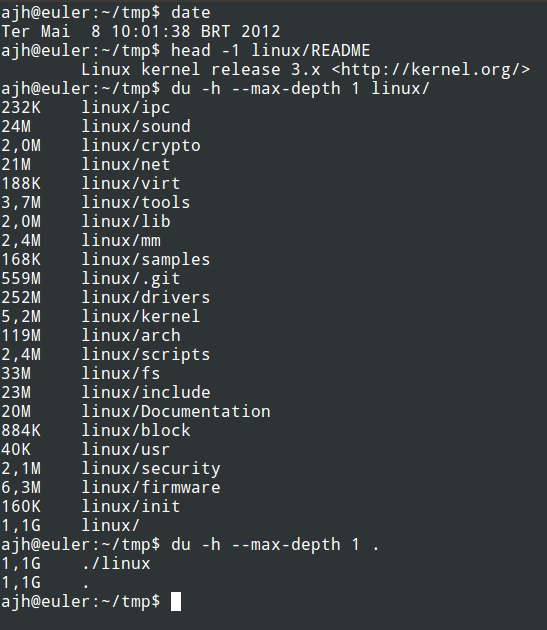
\includegraphics[scale=.275]{../img/linuxsize.png}
  \caption{Captura de tela dos comandos para identificação do tamanho do kernel do GNU/Linux 3.x.}
  \label{fig:kszout}
\end{figure}

O Notebook requisitado, conforme descrito no item~2 da
Tabela~\ref{xls:mpn}, será utilizado pelo Beneficiário do Auxílio para
desenvolvimento dos programas a serem utilizados na Estação de
Trabalho.

\subsection{Orçamentos}

Todos os orçamentos foram anexados na plataforma FAPESP/SAGE e os
nomes dos arquivos estão relacionados ao item na Tabela~\ref{xls:mpn}
na coluna\filbreak ``{\tt referência~do~orçamento}''.
